\subsubsection{Goald}
\label{sec:goald}


\begin{figure}[!htb]
  \centering
  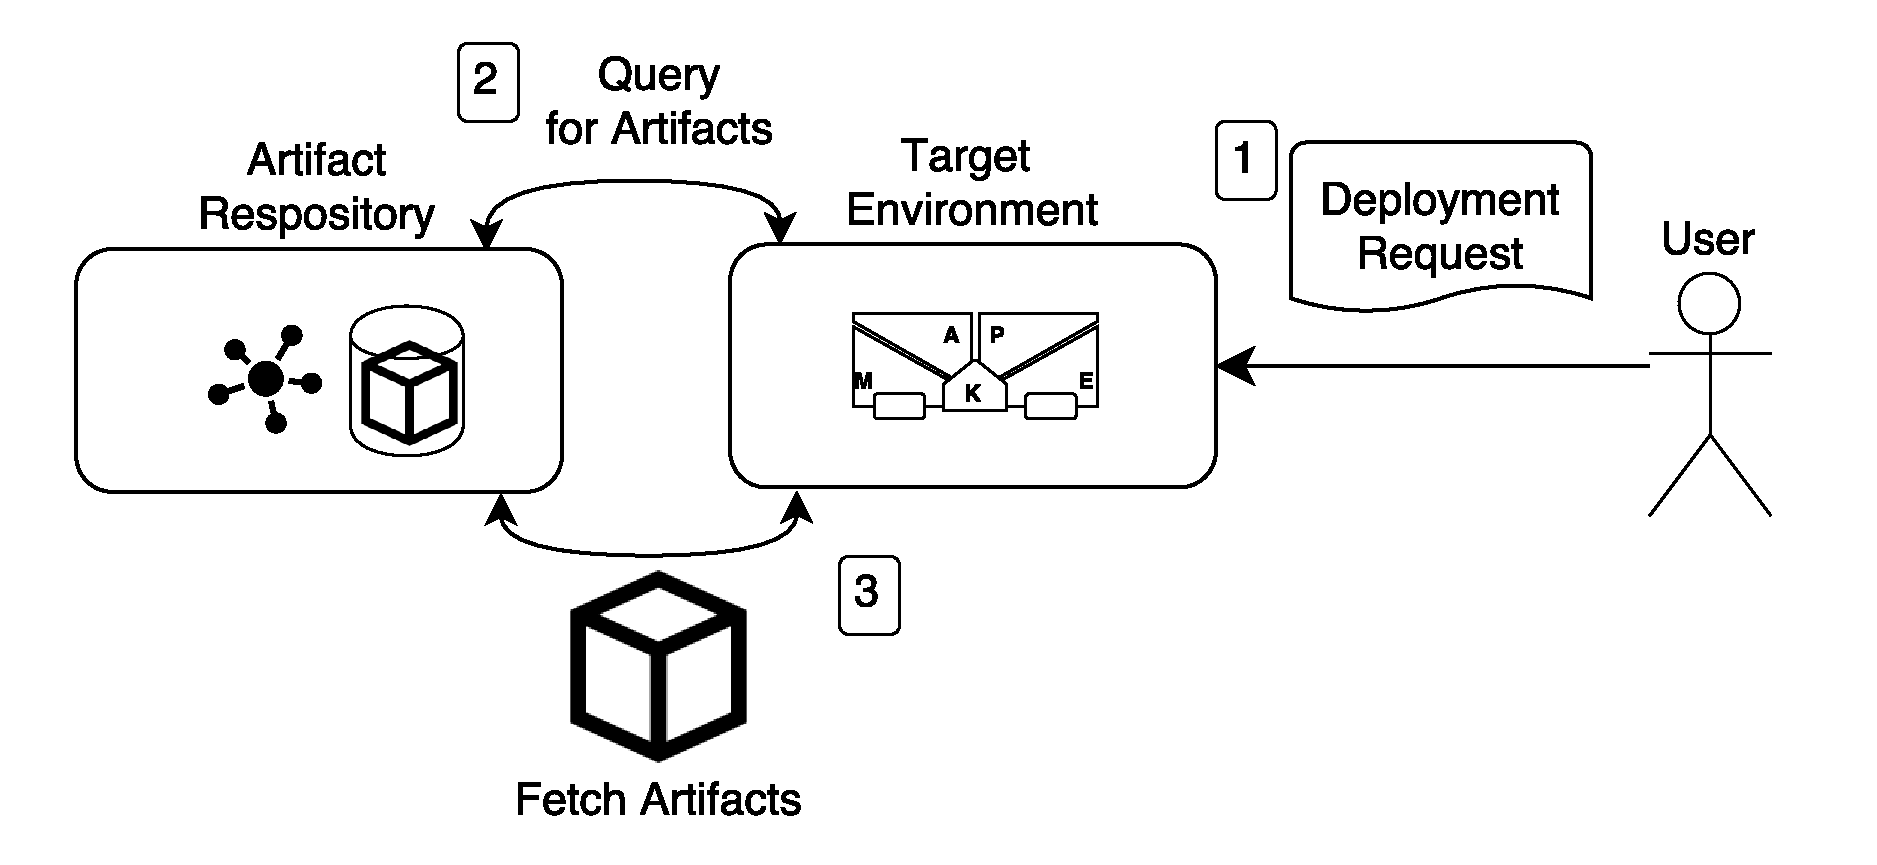
\includegraphics[width=\linewidth]{deployment_actors}
  \caption{Goald Deployment Actors}
\label{fig:deployment_actors}
\end{figure}

Figure~\ref{fig:deployment_actors} depicts the deployment execution. A user interested in using a computing environment to achieve a set of goals submits to this environment which goals it want to achieve in the form of a deployment request.

Then, our system introspect about available computing resources and artifacts present in repository and plan the deployment, generating a deployment plan that is a selection of artifacts that can allow for the goals achievement in the available computing environment. The deployment is them executed by fetching the appropriate artifacts from the repositories.

Facts about the computing environment are directed monitored by the agent by means of sensors. An Artifact should have in its meta-data the condition for its deployment. That condition is specified by a formula of facts.

\subsubsection{Deployment Manager}

Deployment Operations
install
uninstall

\subsubsection{Component Model}
\begin{itemize}
  \item Requirements
  \item Dependencies
\end{itemize}

\begin{itemize}
    \item Information it queries
    \item Listened Events
    \item Dispatched Events
    \item Periodic Execution
\end{itemize}


Life cycle

\begin{figure}[!htb]
  \centering
  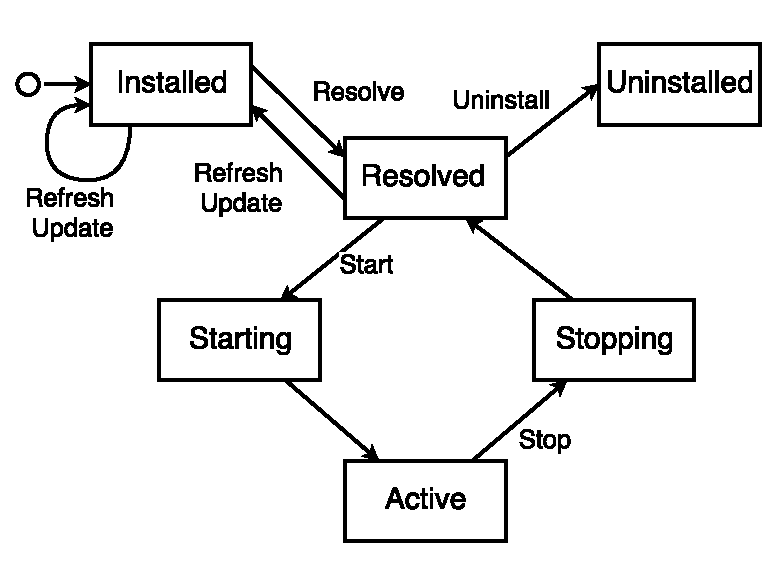
\includegraphics[width=.6\linewidth]{component_life_cycle}
  \caption{Component Life Cycle}
\label{fig:component_life_cycle}
\end{figure}


\begin{itemize}
  \item install
  \item register (listeners)
  \item uninstall
\end{itemize}

Dynamic binding

\subsubsection{Application}

Escalonando a aplicação e o código de adaptação.

\subsubsection{Initial Setup}

Knowledge base,
Component model of the platform: mape-k is in it self a component.



\subsubsection{Illustrative Scenarios}
New Goal

Adapt to resource failure


\subsubsection{Open Adaptation}

\subsubsection{Evolution 1: Notify user about not achievable goals}
If a goal is not achievable a event is generated. With this another component can take action such as notify a external agent (e.g a user) that a goal is not achievable locally with current resources and known components.


\subsubsection{Evolution 2: Adaptive monitoring policies}
% Monitoring policy
A monitor is associated with a monitoring policy that dictate the periodicy that the sense should occur.
\begin{itemize}
  \item periódico:
  \item on demand: Is executed in response to a query
  \item listener: Is called by another system component or external actor.
\end{itemize}



\subsubsection{Addressing Challenges}
RC1 uncertainty at design time and RC2 heterogeneous computing environment

We address these challenges by assembling the system at runtime driven by user goals. Using our approach the developer do not need to know the exact specification of the user environment.
We tackle challenge RC2 (heterogeneous computing environment) using decentralized approach to handle variability of computing environment.

RC3 dynamism
We address this challenge by providing an adaptation framework to handle changes in the computing environment.
Analyzing and responding to changes in the computing environment.

RC4 open adaptation
We address this challenge by providing descentralized approach based on interfaces so that third party developers can provide new components to the system at runtime.


RC5 deployment specification accessible to users
We address this by using goals as abstract way of specifying the system deployment. By this the user do not need to know details about system administration to configure a system. In our approach system administration rules and policies can be implemented as components.
